\newcommand{\secref}[1]{Section~\ref{#1}}
\newcommand{\figref}[1]{Figure~\ref{#1}}
\newcommand{\tabref}[1]{Table~\ref{#1}}
\renewcommand{\eqref}[1]{Equation~(\ref{#1})}

\newcommand{\mbf}[1]{\mbox{{\bf #1}}}
\newcommand{\smbf}[1]{\mbox{{\scriptsize\bf #1}}}
\def\w{\mbf{w}}

%\section{Introduction}
%% {\centering\scriptsize\em
%%   Substantial portions of this text are reproduced from an
%%   author's paper~\cite{friedman:1997:uai}.}

%{\bf Movement Detection from Video:}
Recognizing and tracking moving
objects is one of the main uses of vision.
For computer vision, we can start with `merely' identifying the
foreground.
%first identify what part of each
%frame is due to moving objects.
%(subsequently, separating and tracking
%individuals across frames are also important subproblems)
That is, the task here is to decompose
each frame of video into two parts: all of the moving objects, and
everything else.  Thankfully, in practice, approximate answers are
good enough.  \secref{sec:formal-problem} formally defines the problem,
but first, some background.

For many years, the ``obvious'' approach has
been first to compute some stationary {\em background image}, and then to
identify the moving objects as those pixels in each frame that
differ significantly from the background. We will call this the
{\em background subtraction} approach.
The details of the method are described briefly in
\secref{background-subtraction-section}.

To pick one application, the Roadwatch project at Berkeley,
background subtraction is overall an effective means of
locating and tracking moving vehicles in freeway
traffic~\cite{Koller+al:1994}.
However, in some important cases, background subtraction performs
poorly at vehicle detection: long shadows and heavy traffic.
Shadows move, but treating them as real parts of the vehicles they
overlap leads to many problems, starting with reliably separating each
vehicle from one another.
Moreover, background subtraction tends to treat any
sufficiently slowly changing pixel as
background, which is a problem in heavy traffic because vehicles
then too often disappear into the background.\footnote{Interestingly,
  many predators are also only able to see movement, so that
  it is possible to disappear just by freezing in place.}

These problems are not specific to freeway monitoring, as they arise
from the oversimplified view of the 
general task---detecting moving objects---that
background subtraction takes.  Namely, the approach assumes that
background never changes and foreground always changes.  However,
occasionally-variable background and occasionally-constant
foreground are also possible.  Handling those, when important, needs a
more sophisticated approach; probabilistic techniques prove useful in practice,
especially the use of Expectation-Maximization (EM)~\cite{Dempster+al:1977}.

There is a large literature (several hundred papers in the last
decade, and several annual conferences) on the application
of EM and its family of closely related techniques
to image reconstruction, image segmentation, and
motion identification.   Applications include optical astronomy, laser
range finders, synthetic aperture radar, magnetic resonance imaging, PET, microscopy, and
X-rays.  Almost without exception, EM is used to identify classes of
pixels within an image or classes of motions within an optical flow
field, on the assumption that similar pixels can be grouped
together. Typical examples include Samadani~\cite{Samadani:1995},
Jepson and Black~\cite{Jepson+Black:1993}, Sawhney and
Ayer~\cite{Sawhney+Ayer:1996}, and Weiss and
Adelson~\cite{Weiss+Adelson:1996}.

\subsection{PPAML Motivation}

Interestingly, even just using a simple three-class (``background'', ``darkened'',
``occluded'') mixture model already significantly improves upon
background subtraction for the Roadwatch application~\cite{friedman97uai}.  See
\secref{shadow-and-background-subtraction-section} for a summary of
that approach---which we take as baseline.

The baseline is interesting firstly because it is a natural
probabilistic generalization of the 
classical deterministic approach.
Secondly and more importantly of interest, significant further
improvement should be possible, for example `just' developing and
applying a more complicated probabilistic model should work.

We note, however, that getting inference to work on our suggested baseline
model, on the real application, was not a small amount of
implementation effort.  That severely limited the scope of alternative models we could
feasibly investigate at that time.  A useful probabilistic programming
system would allow a much broader investigation into possible models,
by automating away some of the work presently required when working
from a language with little to no special support for probability.


\subsubsection{Reuse and Tuning}

We expect any implementation to `work' on any video input, although
its performance may be abysmal if some core assumptions are
challenged.  For example, the baseline---and background
subtraction---critically assumes a stationary camera.  A moving camera
will provoke nonsense.

Besides that, while motivated from freeway
traffic, the baseline model and accompanying implementation  make few assumptions.
For example, the model does not assume that all shadows have to point
the same way.  We could have exploited that, and it would have yielded
better segmentations on freeway traffic data.  However, that shadows point the same way is
true only when precisely one light source is relevant.  A window in a
white room is already a situation in which shadows do not behave
simply.  Since we did not build in any such assumption about light
sources, we expect that our model will perform equally at 
identifying and ignoring shadows regardless of the number or geometry of light sources.

We hope that
any effort implementors put into optimizing for some specific
assumptions about the kinds of videos that will be seen is easily
adapted to work well for other situations.  Patient-monitoring in
hospitals and facial-recognition at airports are two such potential applications
where one might expect a foreground-detector trained on freeway data
to still function reasonably well without further massive tuning/training.
It would be interesting to see the results of such cross-domain
application.  How much incremental work is needed by each PPS/team to get
acceptable results as noncritical assumptions change?


\subsubsection{Modularity}

As demonstrated by the existing work, 
reasonably effective performance on the problem is easy enough to
achieve without relying on large, preexisting, machine vision
implementations.  That is helpful for those probabilistic programming
systems that limit callouts to other runtimes.

At the same time, getting the segmentation nearly as correct as a
human in every case has the same structure as presently typical
CAPTCHAs: as complications/noise increase we expect machine vision
systems to break down well before humans do when picking out
objects in images and videos.  If aiming for that or similarly high
levels of performance, then a PPS that permits reuse of
preexisting implementations could easily demonstrate a significant
advantage.


\subsubsection{Space Efficiency}

Video data is an interesting stress test of a PPS.  What is the
overhead the system accrues when representing distributions over
datastructures?  Likely too much by default, since uncompressed video is often large
enough to stress test even deterministic languages.  It will be
interesting to see what answers each PPS provides for working with
models too big to entirely fit in memory all at once.  Is the effort
required to control the PPS's memory overhead more or less than the
effort required to implement probability theory in a deterministic
language?



%% To pick two
%% potential flaws of the reference work: it fails to consider nighttime
%% and deliberately ignores contiguity.
%% Much like shadows, the pixels brightened
%% by vehicles' headlights are easily misclassified as real parts of the
%% vehicles.  Using four classes
%% (``background'', ``brightened'', ``darkened'', ``occluded'') could help.
%% The reference work can be confused by a gray vehicle driving over a
%% gray manhole: it can mistakenly imagine that the manhole remains
%% visible when the vehicle drives over it.  Adding probabilistic contiguity
%% constraints would combat that and many related potential flaws.





%\subsection{Notation}
%\label{sec:notation}


\subsection{Foreground Video Segmentation}
\label{sec:formal-problem}



\subsection{Background Subtraction}
\label{background-subtraction-section}

The roots of background subtraction go back to the 19th century, when
it was shown that the background image could be obtained simply by
exposing a film for a period of time much longer than the time
required for moving objects to traverse the field of view. Thus, in
its simplest form, the background image is the long-term average
image:
\[ B(x,y,t) = \frac{1}{t}\sum_{t'=1}^t I(x,y,t') \]
where $I(x,y,t)$ is the instantaneous pixel value for the $(x,y)$
pixel at time $t$. This can also be computed incrementally:
\[B(x,y,t) = \frac{(t-1)}{t}B(x,y,t-1) + \frac{1}{t}I(x,y,t)\]
The variance can also be computed incrementally, and moving
objects can be identified by thresholding the Mahalanobis distance
between $I(x,y,t)$ and $B(x,y,t)$.

One obvious problem with this approach is that lighting conditions
change over time. This can be handled using a moving-window average,
or, more efficiently, using exponential forgetting. In the latter
scheme, each image's contribution to the background image is weighted
so as to decrease exponentially as it recedes into the past. This is
implemented by the update equation
\begin{equation}
B(x,y,t) = (1-\alpha)B(x,y,t-1) + \alpha I(x,y,t)
\label{forgetting-equation}
\end{equation}
where $1/\alpha$ is the time constant of the forgetting process.
Unlike the moving-window method, this requires no additional storage.
Exponential forgetting is equivalent to using a Kalman filter to track
the background image, as done in~\cite{Koller+al:1994}.




\begin{figure*}[t]
\centering
\subfigure[a]{

\includegraphics[width=0.31\textwidth]{figures/avg.0099.ps}
}
\subfigure[b]{
\includegraphics[width=0.31\textwidth]{figures/img.0100.ps}
}
\subfigure[c]{
\includegraphics[width=0.31\textwidth]{figures/mask.0100.ps}
}
\caption{(a) Background image computed during fast-moving traffic
using exponential forgetting. (b) Current image (frame 100). (c) Thresholded
difference image showing pixels associated with moving objects.}
\label{fast-traffic-figure}
\end{figure*}

\figref{fast-traffic-figure} shows a typical result from the method
operating under favourable conditions. Although there are a few stray
pixels identified as ``moving'' due to image noise, the vehicles are
outlined reasonably well. Standard methods can be used to group the
pixels belonging to each vehicle and to compute and track a smoothed
convex hull.

The sharp-eyed reader will have spotted that the background
subtraction method succeeds not only in detecting moving vehicles, but
also their shadows.\footnote{Some of the road markings are also
labelled as ``moving''---this is due to camera jitter.
Also, the method fails to detect those parts of a moving vehicle that
are approximately the same intensity as the background.
Such problems are unavoidable in any pixel-based method.}
In practice, shadows have been one of the most
serious problems for video-based traffic surveillance in both
commercial and research systems~\cite{Michalopoulos:1991}, sometimes
resulting in undercounting or overcounting by as much as 50\%.  It
might be thought that some simple fix such as lightening or
thresholding might work to eliminate shadows, but these schemes may fail
because parts of the road may be shadowed by buildings, and because of
road markings---a shadow falling on a white line can still result in a
brighter pixel than sunlight falling on tarmac~\cite{Kilger:1992}.

As mentioned in the introduction, another serious problem arises when
objects are slow-moving or temporarily stationary. Here, ``slow-moving''
means that the time of
traversal is non-negligible compared with $1/\alpha$,
the time constant of the exponential forgetting process in
\eqref{forgetting-equation}. When this happens,
the background image becomes corrupted and object detection fails
completely (\figref{slow-traffic-figure}).

\begin{figure*}[t]
\subfigure[a]{
\includegraphics[width=0.31\textwidth]{figures/avg.0924.ps}
}
\subfigure[b]{
\includegraphics[width=0.31\textwidth]{figures/img.0925.ps}
}
\subfigure[c]{
\includegraphics[width=0.31\textwidth]{figures/mask.0925.ps}
}
\caption{(a) Background image computed during slow-moving traffic
using exponential forgetting. (b) Current image (frame 925). (c) Thresholded
difference image showing pixels associated with moving objects.}
\label{slow-traffic-figure}
\end{figure*}

The solution used by Koller {\em et al.}~\shortcite{Koller+al:1994}
was to update the background image with only those pixels
{\em not} identified as moving objects. This is reasonably effective,
but still has problems with very slow traffic because erroneous
pixel classifications perturb the background image, which increases
the number of erroneous classifications, and so on. Essentially, the
distribution of pixels erroneously classified as non-moving is biased
away from the true mean of the background image, causing
instability in the process.

Despite these problems, the idea behind that approach is
essentially right: each pixel must be {\em classified} before being
used to update the background model. The next section shows how this
can be done properly, using a probabilistic classifier and a stable
updating algorithm. This approach also solves the problem with shadows.



\subsection{Probabilistic Shadow and Background Subtraction}
\label{shadow-and-background-subtraction-section}
\label{pixel-model-section}


Consider a single pixel and the distribution of its values over time.
Some of the time it will be in its ``normal'' background state---for
example, a small area of the road surface. Some of the time it may be
in the shadow of moving vehicles, and some of the time it may be part
of a vehicle. Thus, in the case of traffic surveillance, we can think
of the distribution of values $i_{x,y}$ of a pixel $(x,y)$ as the
weighted sum of three distributions $r_{x,y}$ (road), $s_{x,y}$
(shadow), and $v_{x,y}$ (vehicle):
\[ i_{x,y} = \w_{x,y} \cdot (r_{x,y},\ s_{x,y},\ v_{x,y}) \]
These distributions are subscripted
to emphasize that they differ from pixel to pixel; $r_{x,y}$ is a
probability distribution for the way that {\em this specific pixel}
looks when it is showing unshadowed road at the corresponding physical
location. It is essential to have different models for each pixels,
because, for example, some parts of the image may correspond to white road
markings, others to dark streaks in the centers of lanes, and still
others to lamp-posts (see \figref{fast-traffic-figure}).
The weights are also subscripted, because some pixels
may spend more time in shadow or vehicle than others.

\begin{figure*}[t]
\subfigure[a]{
\includegraphics[width=0.23\textwidth]{graphs/intensity-freq.ps}
}
\subfigure[a]{
\includegraphics[width=0.23\textwidth]{graphs/rgb-scatter.ps}
}
\subfigure[a]{
\includegraphics[width=0.23\textwidth]{graphs/intensity-model.ps}
}
\subfigure[a]{
\includegraphics[width=0.23\textwidth]{graphs/rgb-model.ps}
}
\caption{(a) Empirical distribution of intensity values for pixel (160,170)
over 1000 frames. (b) Scatter plot of RGB values for the same pixel.
(c) Fitted three-component Gaussian mixture model for the data in (a).
(d) Scatter plot of 1000 randomly-generated data points from a fitted
three-component Gaussian mixture model for the data in (b).}
\label{pixel-model-figure}
\end{figure*}

Figures~\ref{pixel-model-figure}(a) and~\ref{pixel-model-figure}(b)
show the empirical distribution of intensity and RGB values,
respectively, for pixel (160,170), which is roughly two-thirds of the
way towards the bottom right corner of the image.  These data display
the behaviour one would expect: the shadow and road pixels form two
fairly well-defined peaks, while the vehicle pixels are widely
scattered.  As a first approximation, we assume that each distribution
can be modelled as a Gaussian.  Using expectation maximization, we can fit three-component mixture models to the
data. \figref{pixel-model-figure}(c) shows the fitted model for
intensity values, and \figref{pixel-model-figure}(d) shows a scatter
plot for the fitted RGB model. The fitted models are reasonably good
(but far from ideal) approximations to the empirical data.

%the techniques described in
%\secref{EM-section},
%%
%% the label problem solution is in {results-section}
%%

The model for pixel $(x,y)$ is parameterized by the parameters $\Theta
= \{
w_l, \mu_l, \Sigma_l : l \in \{ r, s, v \}\}$ so that $\w_{x,y} = (w_r,
w_s, w_v )$, $r_{x,y} \sim N(\mu_r,\Sigma_r)$, and so on.%
\footnote{For clarity, we omit the subscript $x,y$ from the names of
these parameters. However, it should be clear that there is a
different set of parameters for pixel position $x,y$.}
Our models apply in two settings. In the first, we examine intensity
levels, and $\mu$ and $\Sigma$ are scalars. In the second, we examine
RGB values, and $\mu$ is a $3\times 1$ vector and $\Sigma$ is a $3\times 3$
matrix. The derivations are identical in the two cases, so we do not
distinguish between them in the following discussion.

Let $i$ be a pixel value (either an intensity level or a vector of RGB
values). Let $L$ be a random variable denoting the {\em label\/} of
the pixel in this image. Our model defines the probability that $L =
l$ and $I(x,y,t) = i$ to be
\begin{eqnarray*}
\lefteqn{P( L = l, I(x,y,t) = i \mid \Theta ) = {}} \\
 & &  w_l \cdot
(2\pi)^{-\frac{d}{2}}|\Sigma_l|^{-\frac{1}{2}} \exp\{-\frac{1}{2}(i -
\mu_l)^T {\Sigma_l}^{-1} (i - \mu_l)\}
\end{eqnarray*}
where $d$ is the dimension of each pixel value (1 or 3 in our case).
Given these probabilities, we can classify the pixel value. Namely, we
choose the class $l$ with highest posterior  probability $P( L = l \mid I(x,y,t)) $.



